\begin{frame}
    \frametitle{Diabetic patient resource consumption analysis}
    \textbf{Too wordy.}
    We will focus our definition of system `cost' on three measures:

    \pause%
    \begin{itemize}
        \item Proportion of total daily admissions
        \item Average length of stay given admission date
        \item Proportion of net costs spent given admission date
    \end{itemize}

    \pause%
    \vspace{10pt}
    These are indicators of resources used and resources necessary.

    \vspace{10pt}
    This grouping by admission date will lead to a degree of misrepresentation
    in our plots.

    \vspace{10pt}
    Allows us to investigate patterns developing over time.
\end{frame}

\begin{frame}
    \frametitle{Resource consumption}
    \textbf{These plots need CIs and accompanying boxplots.}
    \begin{figure}
    \includegraphics[width=\linewidth]{admissions/main.pdf}
    \end{figure}
\end{frame}

\begin{frame}
    \frametitle{Resource consumption}

    \begin{figure}
        \includegraphics[width=\linewidth]{los_time/main.pdf}
    \end{figure}
\end{frame}

\begin{frame}
    \frametitle{Resource consumption}

    \begin{figure}
    \includegraphics[width=\linewidth]{netcost_proportions/main.pdf}
    \end{figure}
\end{frame}
